\item \points{4a} {\bf Compare LoRA and In-Context Learning for XSum}

Plot the few-shot performance of LoRA-16 and in-context learning for XSum in the same plot with the command:

{\small\texttt{python3 main.py --task plot}}

The plot should look as follows:
\begin{center}
    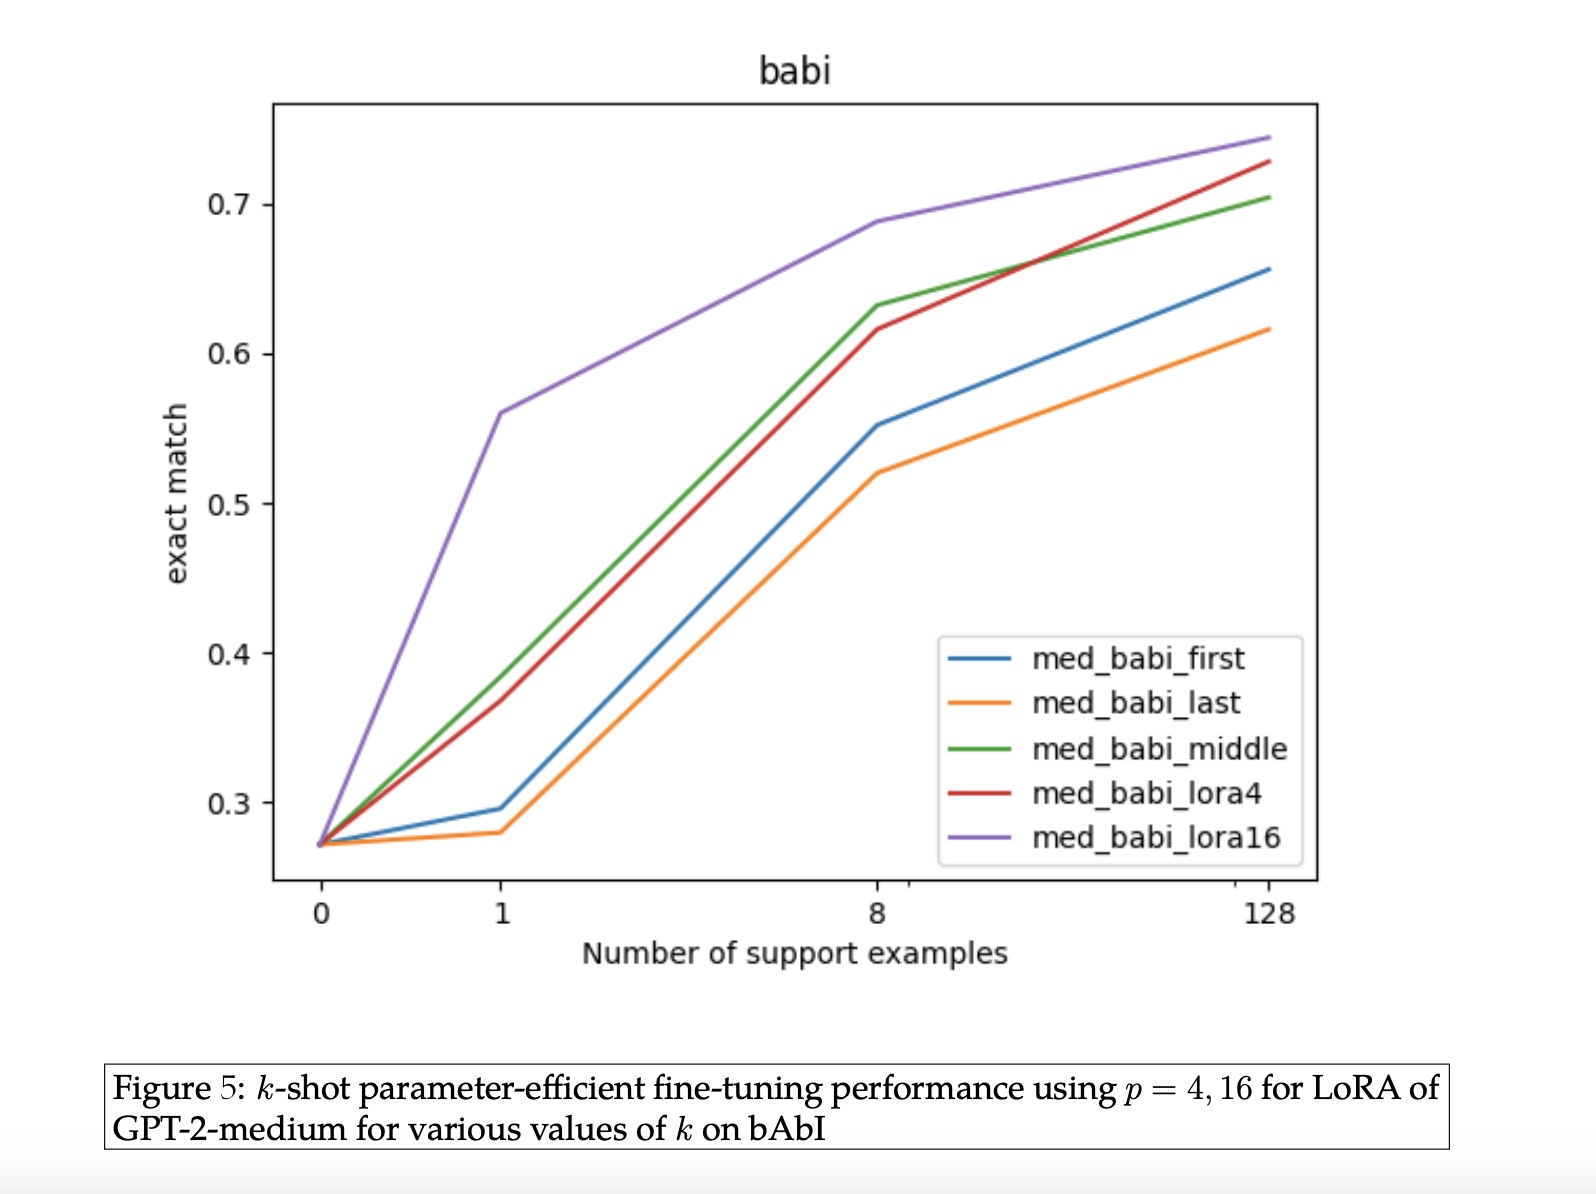
\includegraphics[width=0.75\linewidth]{./figures/compare-4a}
\end{center}

When does in-context learning seem like the better choice, with respect to the amount of data available? What about fine-tuning? What limitation of in-context learning does this result highlight?